\documentclass[titlepage]{article}

\usepackage[margin=1in]{geometry}
% some more shit for the title
\usepackage[T1]{fontenc}
\usepackage{babel}

% Tables and stopping them from displaying in a different section
\usepackage{booktabs}
\usepackage[section]{placeins}

% for inserting images into the document, setting file path, and allowing rotation of inserted images 
\usepackage{graphicx}
\graphicspath{ {./images/} }
\usepackage{rotating}
\usepackage[table]{xcolor}
% mostly just for putting text in math equations
\usepackage{amsmath}
% for aligning the text to the left
\usepackage[document]{ragged2e}

% for inserting hyperlinks in the document, use \url{url} or \href{url}{text}
\usepackage{hyperref}
\usepackage{calligra}
\usepackage[T1]{fontenc}
\usepackage{siunitx}
\usepackage{caption}
\usepackage{multirow}
\usepackage[export]{adjustbox}
\usepackage{tikz}
\usepackage{pgfplots}
\pgfplotsset{soldot/.style={color=black,only marks,mark=*},
	             holdot/.style={color=black,fill=white,only marks,mark=*},
		                  compat=1.12}
\usepackage{paracol}

\begin{document}
\title{\textbf{Lab 5: Resistors in Series and Parallel}}
\author{
    Zachary Pouska\\
    \texttt{001103193}\\
    \and
    Natalie Tran \\ 
    \texttt{000698629}\\ \\
} 

\date{PHYS 236 | Fall 2022\\
Date performed: 24/10/2022}


	\maketitle


	\section{Purpose}
    Familiarity with the behavior of resistors in both series and parallel configurations. Experimental verification of course material and calculations of series and parallel resistors. 

    \section{Materials} 
    \begin{itemize}
        \item Handheld Digital Multimeter (DMM)
        \item Breadboard
        \item Assorted Resistors (270$\Omega$, 330$\Omega$, and 510$\Omega$)
        \item Power Supply
        \item Wires
        \item Alligator Clips
    \end{itemize}


	\section{Theory}	
    In this lab, we make use of the \textbf{ammeter} function in our digital multimeters for the final section. The electrical current is measured in Amperes, which is one coulomb per second ($1.0 A = \frac{1.0C}{1.0 s}$).\\
    \vspace{5pt}
    Additionally, we made use of the most useful feature of a digital multimeter, being the \textbf{voltmeter}. With this mode, our multimeter is able to measure the potential difference between any two points with the units of volts ($\Delta V$), which gives us an idea of the difference in potential energy between two points in our circuit.\\ 

    \textbf{Resistors} have the main property of "resistance", measured in Ohms ($\Omega$), which can be thought of as a ratio of Volts over Amperes, or how many volts will be dropped across the resistor for a certain amount of current. 




    \subsection*{Resistors in series}
        $$R_{eq} = R_1 +R_2 + R_3 $$
        The total Voltage across resistors in series is equal to the sum of voltage drops across each subsequent resistor. $$ V_{eq} = \varepsilon = V_1 + V_2 + V_3 = I R_1 + I R_2 + I R_3 $$

    \subsection*{Resistors in parallel} 
        $$R_{eq} = \left( \frac{1}{R_1} + \frac{1}{R_2} + \frac{1}{R_2} \right)  $$
        The voltage drop across each resistor in a parallel setup is equal to the potential difference of the battery $\varepsilon$.
        $$V_{eq} = \varepsilon = V_1 = V_2 = V_3 $$


	\section{Experiment Analysis}
    When we have resistors in parallel, the potential difference across them are the same. 
    



	\section{Procedure}
        \subsection{Measurement of the resistors using DMM}

            \begin{figure} 
                \centering
                \caption{Six unknown resistors on a breadboard}
                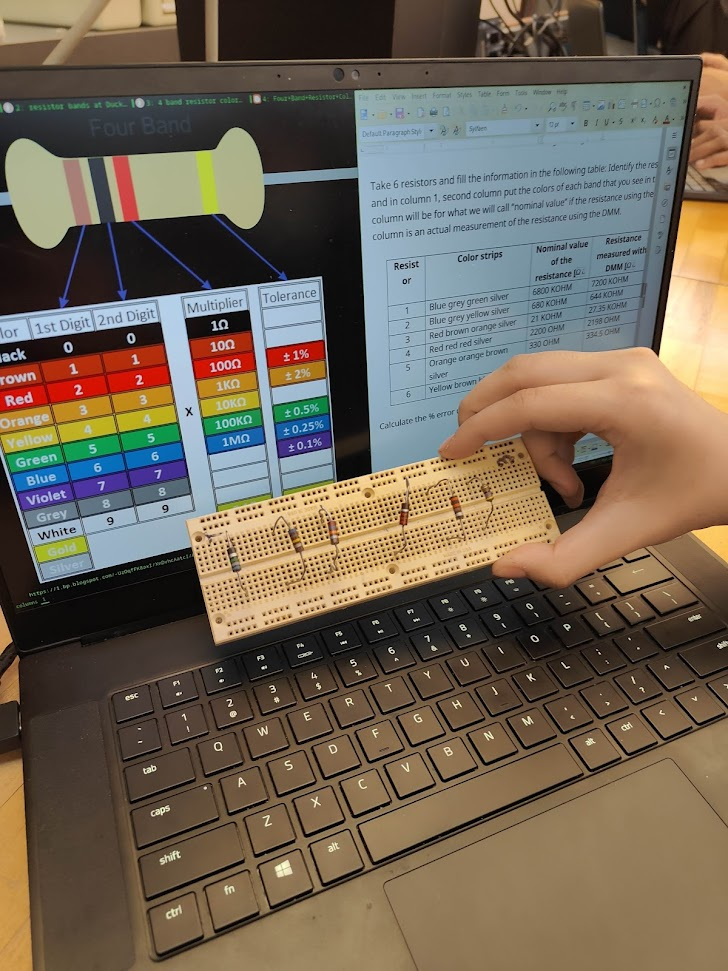
\includegraphics[scale=0.2]{procedure/unknownresistors}
            \end{figure} 


        \subsection{Series Circuit}

        \begin{figure} 
            \centering
            \caption{Resistors in a series configuration}
    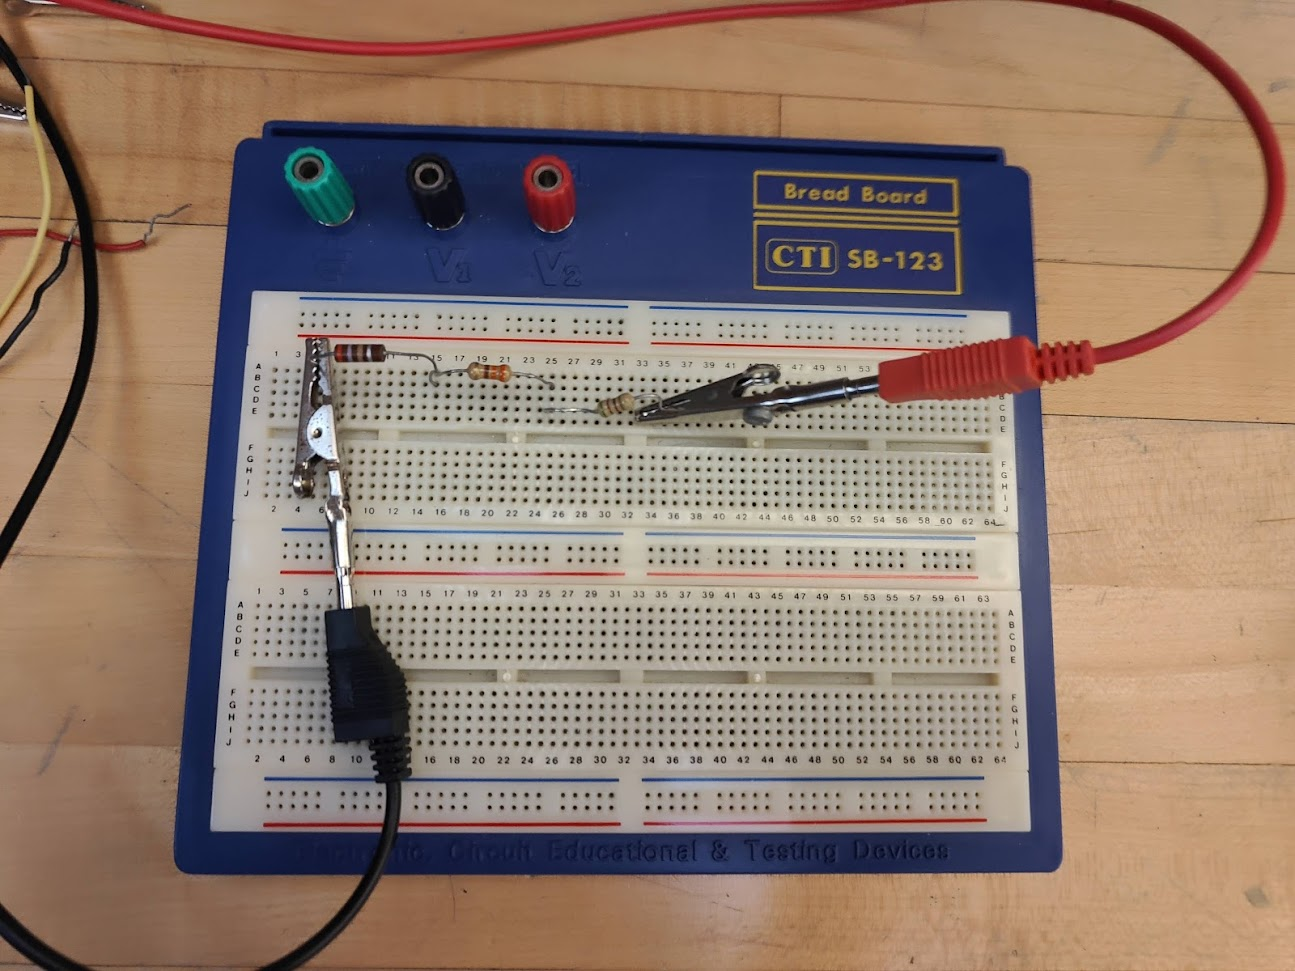
\includegraphics[scale=0.2]{procedure/series} 
        \end{figure}

        \subsection{Parallel Circuit}

        \begin{figure} 
            \centering
            \caption{Resistors in a parallel configuration}
            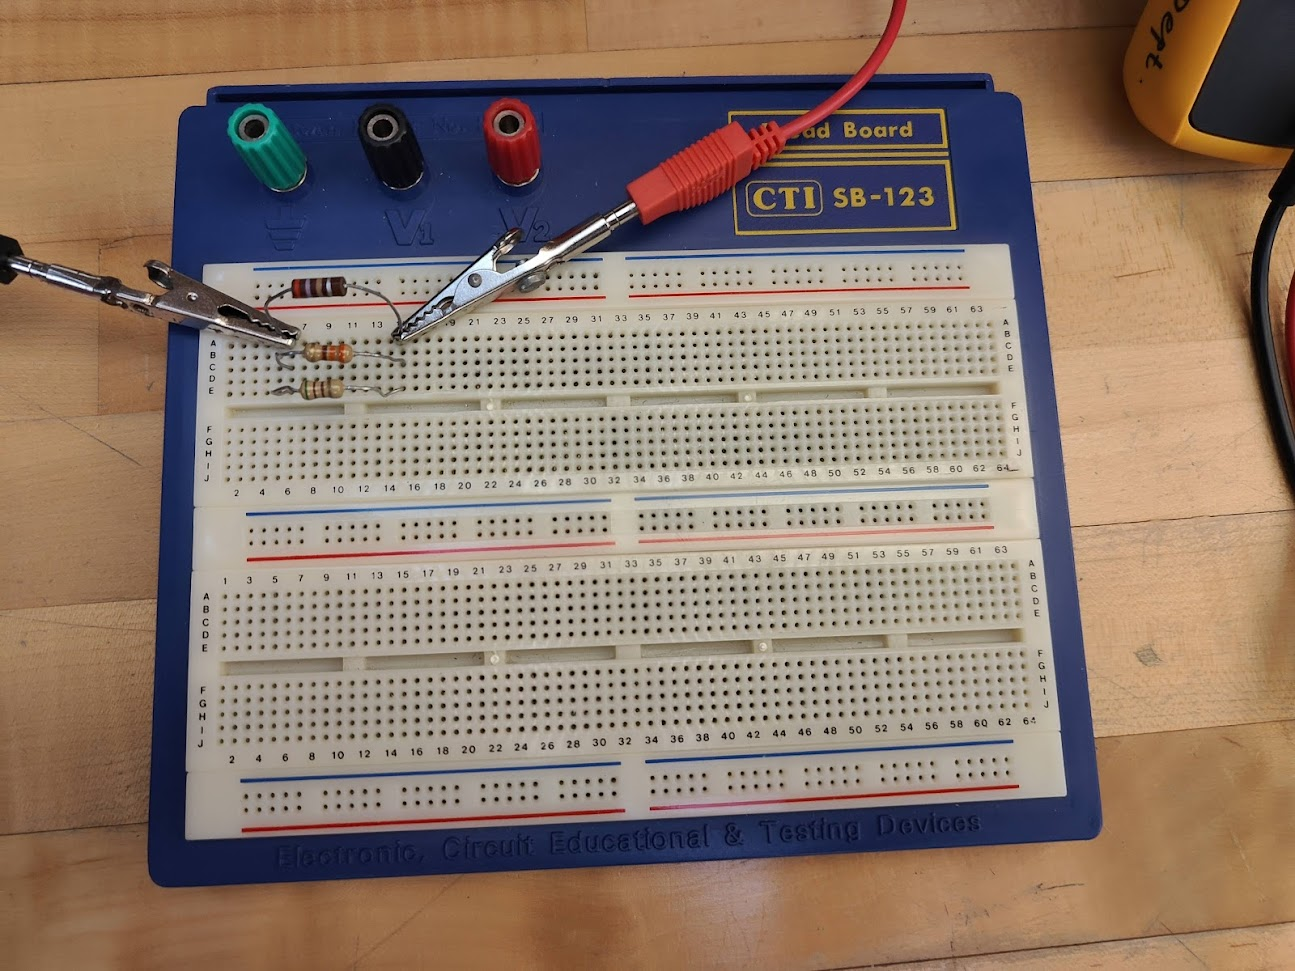
\includegraphics[scale=0.2]{procedure/parallel} 
        \end{figure}



	\section{Data and Graphs}
	\subsection{Part 1}
	\subsection{Part 2} 
	\subsection{Part 3}
    \section{Calculations \& Results}

        \subsection{Part 1} 
    For calculating the equivalent resistance

        \subsection{Part 2} 


	\section{Questions}



    \begin{figure} 
        \centering
        \caption{Series and parallel circuit diagram}
        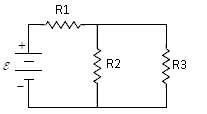
\includegraphics[scale = 1.2]{images/questions/circuit.png}


    \end{figure}

	\section{Conclusion}

\end{document}
